\documentclass[tikz,border=5pt]{standalone}
\usepackage{times}
\usepackage{amsmath,amssymb}
\usetikzlibrary{positioning,fit,arrows.meta,backgrounds,shapes.geometric,calc,shadows,decorations.pathreplacing}

\begin{document}
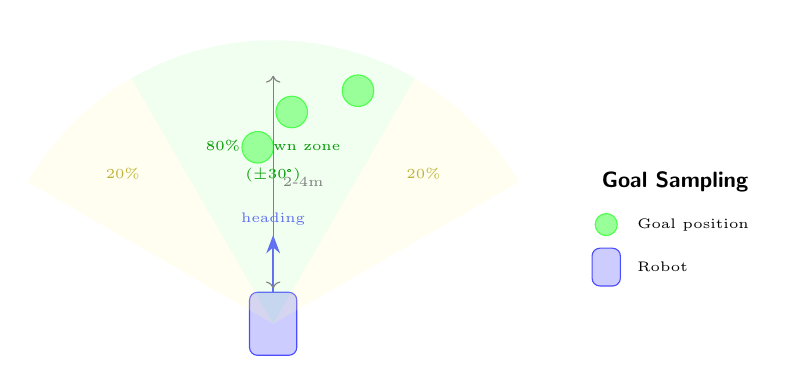
\begin{tikzpicture}[
    scale=0.9,
    robot/.style={draw=blue!70, fill=blue!20, minimum width=0.6cm, minimum height=0.8cm, rounded corners=1mm},
    goal/.style={draw=green!70, fill=green!40, circle, minimum size=0.4cm},
    zone/.style={draw=none, fill opacity=0.2},
    arrow/.style={->, >=Stealth, thick}
]

% Robot
\node[robot] (robot) at (0,0) {};
\draw[arrow, blue!70] (robot.north) -- ++(0,0.8) node[above, font=\tiny] {heading};

% Forward cone (80% at spawn)
\fill[zone, fill=green!30] (0,0) -- (60:4) arc (60:120:4) -- cycle;
\node[font=\tiny, green!60!black] at (90:2.5) {80\% spawn zone};
\node[font=\tiny, green!60!black] at (90:2.1) {($\pm$30\textdegree)};

% Forward hemisphere (20% at spawn, 65% after reaching)
\fill[zone, fill=yellow!30] (0,0) -- (30:4) arc (30:60:4) -- cycle;
\fill[zone, fill=yellow!30] (0,0) -- (120:4) arc (120:150:4) -- cycle;
\node[font=\tiny, yellow!70!black] at (45:3) {20\%};
\node[font=\tiny, yellow!70!black] at (135:3) {20\%};

% Goals
\node[goal] at (85:3) {};
\node[goal] at (95:2.5) {};
\node[goal] at (70:3.5) {};

% Distance annotations
\draw[<->, thin, gray] (0,0.5) -- node[right, font=\tiny] {2-4m} (90:3.5);

% Legend
\node[font=\sffamily\footnotesize, anchor=west] at (4.5,2) {\textbf{Goal Sampling}};
\node[goal, scale=0.7] at (4.7,1.4) {};
\node[font=\tiny, anchor=west] at (5,1.4) {Goal position};
\node[robot, scale=0.6] at (4.7,0.8) {};
\node[font=\tiny, anchor=west] at (5,0.8) {Robot};

\end{tikzpicture}
\end{document}
